\chapter{Usage samples}
\label{cha:sample}
At this point, we can start using the package functionalities to retrieve some data 
from the Service Providers we chose and make some analysis from which we shall
extract useful information.

\section{Block size}
The Block size was the primary reason for the Hard Fork on August 1$^{st}$, 2017. Orginally,
the dimension of Bitcoin's blocks was of 1 MegaByte and in order to increase the 
scalability of the network, with Bitcoin Cash, it has been raised to 8 MegaBytes.
A relevant analysis could be done by inspecting all the blocks to 
get the real size of each mined block since the BCH Hark Fork.

\begin{figure}[h]
    \centering
    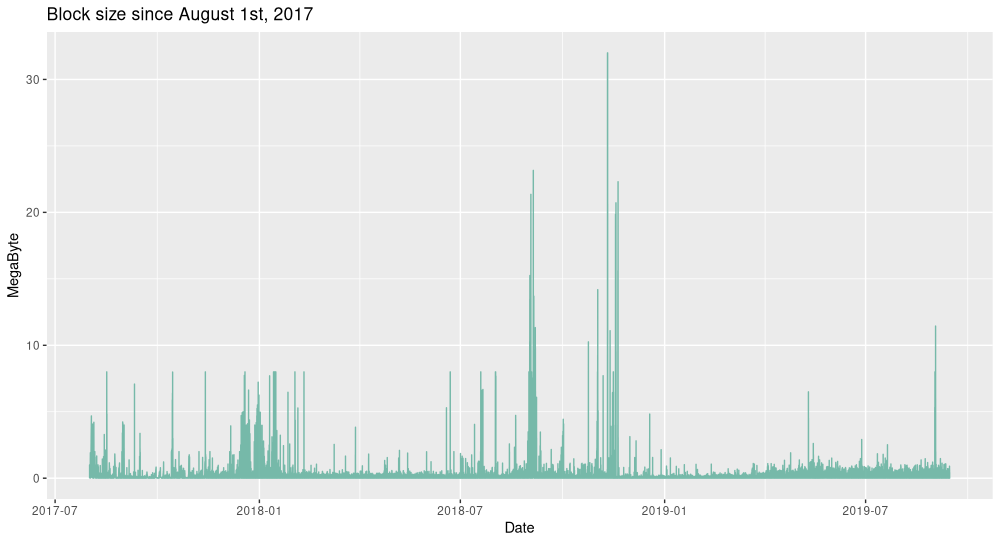
\includegraphics[width = 0.9\textwidth]{blocksize2.png}
    \caption{Graph of the dimension of each mined block since August 1$^{st}$, 2017}
    \label{fig:request}
\end{figure}

Thanks to this Graph, it is possible to determine that almost one year later, the block 
size has incremented again bringing the dimension of a block up to 32 MegaBytes. 
But, even if there is a lot of space in each block, it is not entirely used, 
actually for the most of the time is used just a small portion of its capacity.\\
\pagebreak

\section{Transactions}
Growing the block size, was only a mean for increasing the number of the transactions 
in each block. Thus, not only the scalability has been improved, but also the fees for every 
transaction have been lowered.

\begin{figure}[h]
    \centering
    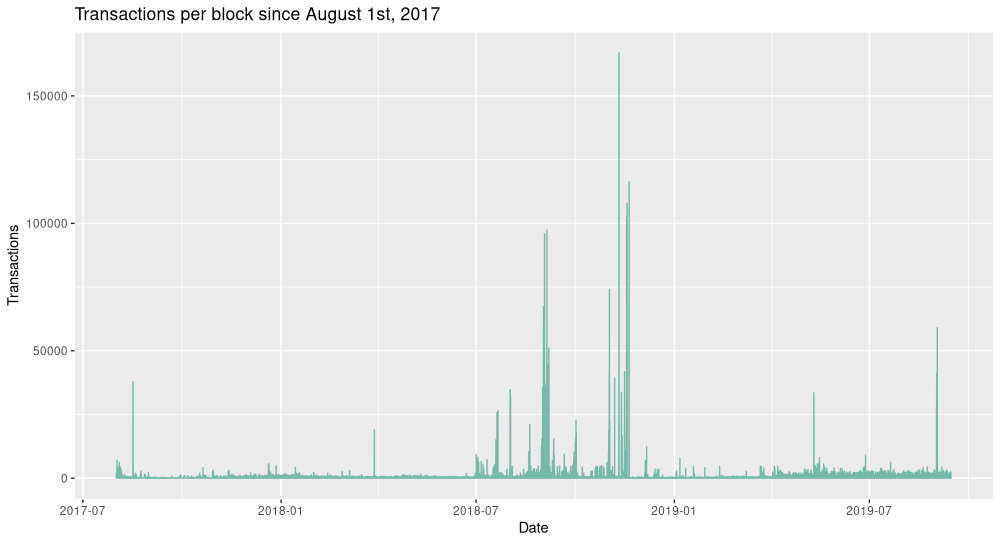
\includegraphics[width = 0.9\textwidth]{transactions1.png}
    \caption{Graph of the number of transactions per block since August 1$^{st}$, 2017}
    \label{fig:request}
\end{figure}

By watching the above graphs it is possible to see and to analyse the behaviour of the transaction count
related to the size of each block. Moreover, a comparison shall be made between Bitcoin and Bitcoin Cash throughput.
The BTC network can handle a maximum of 7-8 TPS\cite{thecryptonomist}. Meanwhile, by reading 
the graph and by making a little bit of math, the throughput of the Bitcoin Cash network can be estimated. 
Considering that a block is mined every 10 minutes, the formula to find the throughput is: 

$TPS = Transactios per block / minutes per block / 60 seconds$. \\\\
The above graph shows that the BCH throughput is more than: $150.000 / 10 / 60 = 250 TPS$

\section{Mining Pools}
As already mentioned, the consensus algorithm adopted by Bitcoin Cash is the Proof of Work.
With the growing of the Bitcoin Cash network, also the number of miners has grown. In fact, 
there is a massive electricity consumption for the mining process. That leads also to a 
massive computational power. Furthermore, trying to mine a block as an individual is a waste of
resources, because, by comparing your computational power with the one of the entire network, your
probability to close a block before the entire network is extremely low. For this reason 
mining pools have been created. In this way, if someone wants to participate at the mining process,
he/she has just to join a mining pool where all the computational power of the participants is combined.
At this point, the probability for a pool to mine a block is much more, and in case it succeeds in 
closing a block, the rewarding is distributed to all the participants proportionally to their computational power.\\
\pagebreak

\begin{figure}[h]
    \centering
    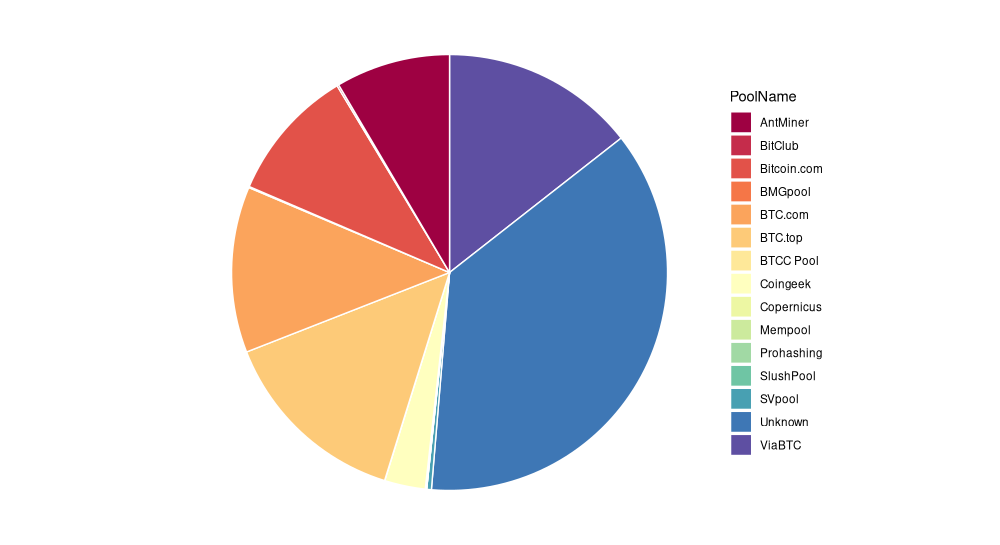
\includegraphics[height = 7cm]{poolminers.png}
    \caption{Proportion of the mined blocks since Auguts 1$^{st}$, 2017 by each mining pool}
    \label{fig:request}
\end{figure}

In the graph above, we can see in proportion how many blocks have mined every mining pool and
how many pools joined in mining Bitcoin Cash ever since his birth.\\
With the next graph, we can extend the analysis of the mining pools by spreading them over the time.
By doing so, we can also have an overall idea on how much computational power each pool spent 
in a specific period.

\begin{figure}[h]
    \centering
    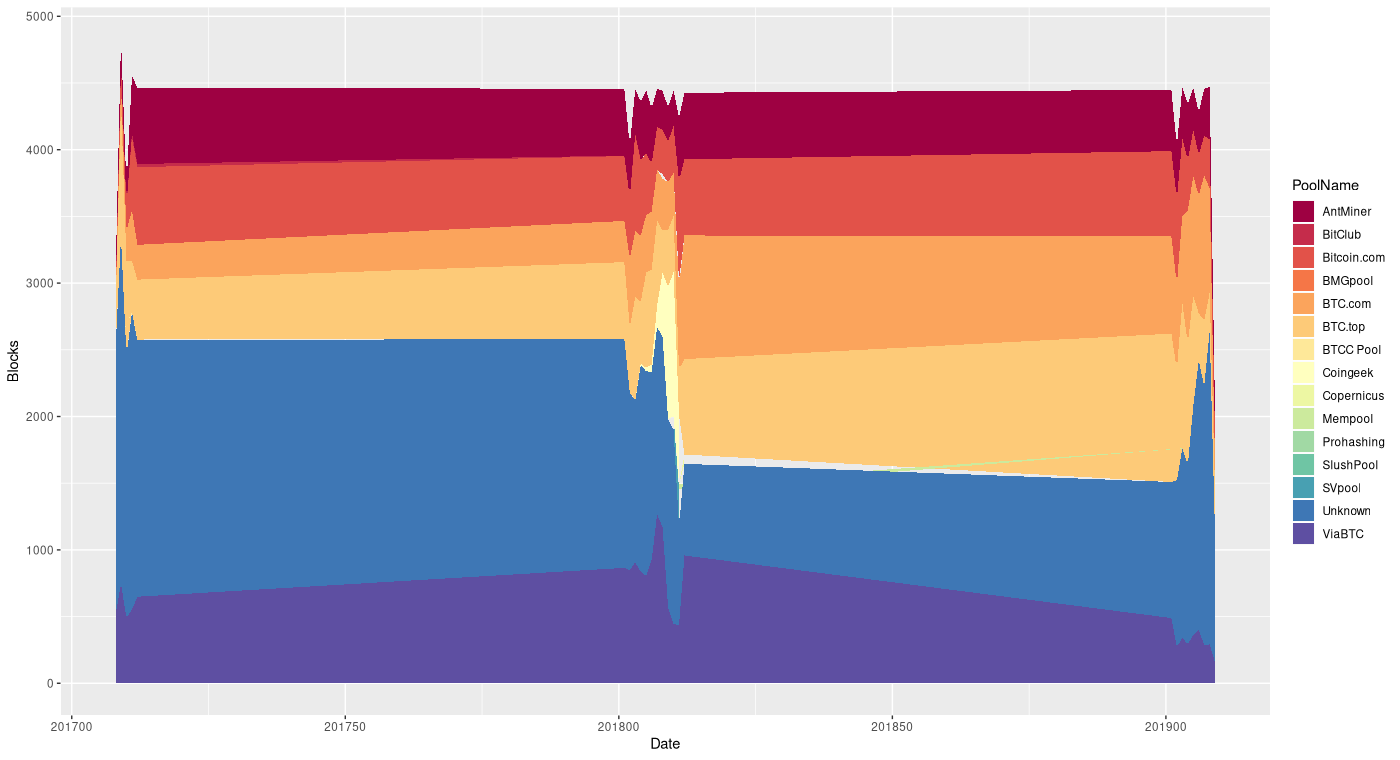
\includegraphics[width = 0.9\textwidth]{stackblocks.png}
    \caption{Number of blocks mined by each mining pool since August 1$^{st}$, 2017}
    \label{fig:request}
\end{figure}

\section{Conclusion}
I am satisfied with the possibilities of data analysis this implementation gives to
anyone that wants to take a look at the Bitcoin Cash blockchain.
The work done for this thesis gave me a chance to go deeper into the history and the 
working mechanism underlying the blockchain technologies. Furthermore, by going 
deeper into the study of this kind of technology, I feel I gained enough knowledge 
to be able in the future to develop new applications based on it.

